%%%%%%%%%%%%%%%%%%%%%%%%%%%%%%%%%%%%%%%%%%%%%%%%%%%%%%%%%%%%%%%%%%%%%%%%%%%%%%%
%2345678901234567890123456789012345678901234567890123456789012345678901234567890
%        1         2         3         4         5         6         7         8

\documentclass[letterpaper, 12 pt, conference]{ieeeconf}  % Comment this line out
                                                          % if you need a4paper
%\documentclass[a4paper, 10pt, conference]{ieeeconf}      % Use this line for a4
                                                          % paper

\IEEEoverridecommandlockouts                              % This command is only
                                                          % needed if you want to
                                                          % use the \thanks command
\overrideIEEEmargins
% See the \addtolength command later in the file to balance the column lengths
% on the last page of the document

\usepackage[utf8]{inputenc}
\usepackage[T1]{fontenc}
\usepackage{graphicx}
\usepackage{float}


% The following packages can be found on http:\\www.ctan.org
%\usepackage{graphics} % for pdf, bitmapped graphics files
%\usepackage{epsfig} % for postscript graphics files
%\usepackage{mathptmx} % assumes new font selection scheme installed
%\usepackage{mathptmx} % assumes new font selection scheme installed
%\usepackage{amsmath} % assumes amsmath package installed
%\usepackage{amssymb}  % assumes amsmath package installed

\title{\LARGE \bf
Music Genre Classification of Closely Related Sub-Genres 
}

\author{ \parbox{2 in}{\centering Christopher Calloway
        % \thanks{}\\
        Electrical Engineering\\
       Stanford University\\
        {\tt\small cmc2374@stanford.edu}}
        \hspace*{ 0.5 in}
        \parbox{2 in}{ \centering Yiwen Jiang\\
        % \thanks{}\\
        Electrical Engineering \\
        Stanford University\\
        {\tt\small yjiang98@stanford.edu}}
          \hspace*{ 0.5 in}
        \parbox{2 in}{ \centering Louise Zhuang\\
        % \thanks{}\\
        Electrical Engineering \\
        Stanford University\\
        {\tt\small llz@stanford.edu}}
}

% \author{ Chris Calloway$^{1}$, Yiwen Jiang$^{2}$, Louise Zhuang$^{3}$% <-this % stops a space
% \thanks{* Supervised by Mert Pilanci, Yifei Wang}% <-this % stops a space
% \thanks{$^{1}$ Chris Calloway
%         {\tt\small cmc2374 at stanford dot edu}}%
        
% \thanks{$^{2}$ Yiwen Jiang
%         {\tt\small  at stanford dot edu}}%

% \thanks{$^{3}$ Louise Zhuang
%         {\tt\small  at stanford dot edu}}%
        
    
% }


\begin{document}



\maketitle
\thispagestyle{empty}
\pagestyle{empty}


%%%%%%%%%%%%%%%%%%%%%%%%%%%%%%%%%%%%%%%%%%%%%%%%%%%%%%%%%%%%%%%%%%%%%%%%%%%%%%%%
\begin{abstract}

This report presents our attempt at training machine learning models to predict music sub-genre labels of closely related musical genres. Musical genres, at their core, are subjective categorical labels based on human perception and consensus. Despite this subjectivity, musical genre classification using broader genres (such as rap, rock, classical and jazz) has had much success using models such as KNN, SVM and neural networks (NN). Our goal was to see if such methods could extend to closely related genres  which we call sub-genres of music. We find that such methods are effective but more work needs to be done to achieve even higher accuracies. 




\end{abstract}


%%%%%%%%%%%%%%%%%%%%%%%%%%%%%%%%%%%%%%%%%%%%%%%%%%%%%%%%%%%%%%%%%%%%%%%%%%%%%%%%
\section{INTRODUCTION}

\subsection{Overview}

Music genres are subjective labels critics and consumers alike put on music for categorization purposes. 
As a consequence of this subjectivity, the labeling of genres is often controversial and a point of discussion among listeners. 

Nonetheless, to a lay observer, what distinguishes rock and roll music from classical music is sonically and empirically obvious. Thus it isn't terribly surprising that machine learning methods for the classification of broad musical categories (rap, rock and roll, classical, jazz, etc) yield results in excess of 89\% \cite{c1, c2, c3}. Thus despite the subjectivity of music labels, there is enough data within audio samples for both humans and machines alike to confidently classify music into broader genres.

But what about more closely related genres? In other words, what happens when we remove the assumption of broad genres for music genre classification and instead use niche genres of music with only slight sonical differences?  To answer this, we attempt to train machine learning models on very closely related sub-genres of music. 

In this paper we consider the following sub-genres of closely related music: Shoegaze vs. Dream pop, Math rock vs. Post rock, Roots rock vs. Folk rock, and Progressive house vs. Tech house. We pick these genres because fans and critics alike are split on what exactly defines the difference between these sets of genres. Can machine learning methods find such the distinction? 

Before attempting to answer this, we make a critical assumption. We assume that there is a ground truth sub-genre label for these sub-genres. To that end, we get this ground truth label from the artist's record label. The record label for an artist is what officially assigns a genre to a particular album, and they do so without regard to any fan or critical debate of the accuracy \cite{c8}. Thus this gives us a solid ground truth label to build our dataset upon. Thus, our training data is then a collection of these officially labeled albums from various artists and record labels.

After collecting and pre-processing our data, our results indicate that we can get accuracies upwards of 83\%  for classifying closely related sub-genres. The best results occur for NN approaches, but results upwards of 77\% were also achieved for KNN and SVM approaches. Our results indicate a need for larger datasets, but also indicate that neural networks are a promising approach for music sub-genre classification. 




\subsection{Related Work}


There has been lots of work in the field of machine learning approaches to music genre classification. As mentioned in the overview, the results of various machine learning classifiers is upwards of 89\%, with the best being convolutional neural networks (CNN),  such as \cite{c4}. 

However, there has been less work in looking at very niche sub-genre classification. One such attempt was made to classify Metal sub-genres in \cite{c5}. In this paper, 30 second samples of songs from sub-genre-specific Spotify playlists were taken for various metal sub-genres such as Black metal and Thrash metal. The audio data was then converted into Mel spectrograms. This data was split into 80\% training data and 20\% testing data and then was fed into a convolutional recurrent neural network. After training, the network was able to predict metal sub-genres on the test set with a 62\% accuracy. 

In another paper, decision trees, random forests, extremely randomised trees, and gradient tree boosting were used to classify 23 related EDM sub-genres \cite{c6}. The authors were able to achieve an accuracy of 59\% without any neural networks involved. 

In another paper about classifying 3 sub-genres of jazz, Neural Networks, linear SVM and KNN were used to classify the sub-genres. The authors were able to achieve classification accuracies of 79.39\%, 67.12\%, and 77.43\%  respectively \cite{c7}. The authors also found that adding a multi-layer perceptron network before a long short-term memory layer in their neural network boosted the accuracy to 89.824\%.

From this related work, we concluded that a neural network model looked the most promising in terms of accuracy. However, we also determined a KNN and SVM model were likely to produce sufficient results based on the success of \cite{c7}. The work done on decision trees, and random forest models did not seem to be successful enough to warrant an attempt. Thus from this review, we decided to train a KNN, SVM, and NN model for each sub-genre. Furthermore, we found the Spotify data collection method in \cite{c5} to be a promising approach for our own data collection. We discuss this more below.




\section{PROCEDURE}


\subsection{Data collection}


Similar to \cite{c5}, to train our model we collected albums of songs using the Spotify API from genre labeled Spotify playlists. Spotify’s API came with a number of constraints and useful features.

A major constraint is that the API only allows a random 30 seconds of raw audio data to be downloaded to an MP3 format. While this was limiting, it did simplify the feature extraction part of pre-processing since there was no ambiguity as to how long the audio sample should be or which portion of the song to pull from. A useful feature of the Spotify API is that it provides its own audio features for songs such as key, tempo, loudness, acousticness, danceability, and instrumentalness. The challenge with these features is figuring out how to normalize the values (including strings) and also understanding the quantitative nature of these measurements. For instance, it is not clear in the Spotify API documentation what the quantitative measure "danceability" really is. For these reasons we did not use these features in our model training; however, we collected them in our database anyways for potential future work. Another limitation of the Spotify API is that not every song has a 30 second raw audio data preview and some do no not have the other audio features mentioned above. It is unclear why some songs do not have these, but for our data collection we simply rejected any songs that lacked either of these.


Spotify playlists are a convenient way of collecting data so that Spotify API requests can easily pull data from them. Unlike \cite{c5}, we did not use pre-existent Spotify playists for our labeled data. Instead, we created our own Spotify playlists based on the genre labels given by the artist’s record label. The full methodology to generate a playlist is described step by step below. 

\begin{enumerate}
    \item Select a genre. For instance, "Dream pop"
    \item Find a comprehensive list of artists for a specific genre. Wikipedia has good articles for this, for example the "List of Dream pop artists" article
    \item Pick an artist from the list at random that was not already picked
    \item Find the first album the artist released in which the record label gave the album the desired genre
    \begin{enumerate}
        \item If the record label gave it multiple genres, including the genre we are comparing against, for example Dream pop and Shoegaze, we reject it and move on to the next album in the artist's discography. If there are no relevant albums left, then move back to step 3
        \item Else, if the record label gave it multiple genres that don't overlap with what we are comparing against, for instance Dream pop and Ethereal pop, we allow it and add all the songs on the album to the Spotify playlist and then move to back to step 3
        \item If the record label genre exactly matches (for instance just Dream pop) then we add all the songs on the album to the playlist
    \end{enumerate}

    \item We repeat from step 3 until we have 600 songs in our playlist
    \item We repeat from step 1 until we have playlists for each genre
    \item Finally we use the Spotify API to download the 30-second MP3 samples and other audio features for each song in each playlist and store them in .npy files.
\end{enumerate}

There are a couple of important caveats to the above procedure that are worth mentioning. For any album that was collected, every song on the album was added. The only exceptions were that remixes and non-musical content (e.g., interviews) were excluded. Furthermore, an artist could only appear once per playlist. However, nothing prohibited an artist from appearing in multiple playlists. Thus it was possible the same artists could appear in both the Dream pop and Shoegaze playlist, or any other playlists. Lastly, in some cases there were not 600 songs available on Spotify for a sub-genre. The total number of songs downloaded to our data base using the Spotify API per genre are outlined below. Note that none reach 600 since we removed any songs that did not have 30-second previews or audio feature data.

\begin{enumerate}
    \item Dream pop: 577
    \item Shoegaze: 578
    \item Math rock: 578
    \item Post rock: 580
    \item Folk rock: 169       
    \item Roots rock: 193
    \item Tech house: 349
    \item Progressive house: 360
\end{enumerate}

Finally this data was split into 70\% train, 20\% validation, and 10\% test. Before training the models, the following pre-processing was done.


%  OLD VERSION:
 

%To train our model we collected specifically genre labeled data from Spotify. 578 shoegaze songs and 577 dreampop songs, as labeled by the Record Label of their containing album, were collected and downloaded using the Spotify API.
% The Spotify API only allows a random 30 seconds of the song to be downloaded so all such songs were 30 second samples taken at a random interval. When adding  songs, we added them by the entire album, only excluding songs that did not have 30 second samples or other such audio features and remixed songs from other artists if applicable.

% Not all songs were strictly "dreampop" or strictly "shoegaze". For example some were labled as "dreampop and etheral pop" or "shoegaze and noise rock". We allowed for such genre blends in our dataset. However, an album that was labeled as "dreampop and shoegaze" was not allowed. We restricted our dataset to allow only one album per artist to encourage a varkety of artists in our database. To determine which album to add to the database we picked the earliest released album with the proper label. Note that in some cases an artist would have a release as "shoegaze" and perhaps later in their discography a release as "dreampop". We allowed for this, so in some cases an artist appears in both the shoegaze and the dreampop datasets with different albums. 

% After the sample songs were downloaded, the mp3 data per genre was read and stored into on large matrix. This large and randomly split 70\% train samples and 30\% test samples. These samples were then stored in .npy files.

\subsection{Data Pre-Processing and Feature Extraction}


From the .npy files, MFCCs were extracted as features from each data sample for training the KNN and SVM models. MFCCs (Mel-Frequency Cepstral Coefficients) are one of the most commonly used features for audio and speech recognition machine learning purposes. MFCCs provide more reliable spectral estimations for audio signals compared to straightforward spectral transformations. 

The calculation of MFCCs takes into account the characteristics of audio signals as well as human hearing. Since music genres are human perceived labels, such an audio feature was appropriate for our models. For MFCCs, signals are framed into shorter frames to account for the constantly changing nature of audio signals. The calculation of power spectrum and use of Mel filter bank mimic human hearing where different emphasis is put on different ranges of frequencies. This is represented in wider bands used at higher frequencies, as the focus is on energy rather than variation, whereas it is the opposite for lower frequencies. The final coefficients are obtained through calculating the Discrete Cosine Transform coefficients of the logarithm of the filter bank energies. 

For our purpose, the original MP3 files were read in with sampling rate of Fs = 22050 Hz, thus each 30-second data sample had length of 661500. Sixteen MFCCs were used, with frame length of 2048 and hop length of 512 samples. 

With the given MFCC feature parameters, for each audio sample, we obtain 16 MFCCs with length of 1288. Using the output MFCCs directly would result in heavy computational load. To reduce this load, the coefficients for each window were then flattened into a one-dimensional sequence, and principal component analysis (PCA) was performed to reduce the dimensionality of the data. PCA compresses data by maintaining feature information in the dimensions of highest variance, thus preserving key information about the Mel spectral features while also de-noising the data, which improves classification accuracy.


\subsection{KNN Design}

Initially, a k-nearest neighbors (KNN) classifier was used to classify thirty-second song samples between two subgenres. 
Classification of a test sample was determined by the mode of the k closest samples from the training data in the feature space, as shown in Figure \ref{fig:knnimg}. The Euclidean (L2) distance metric was used to determine closeness for this project.
\begin{figure}[!ht]
  \centering
  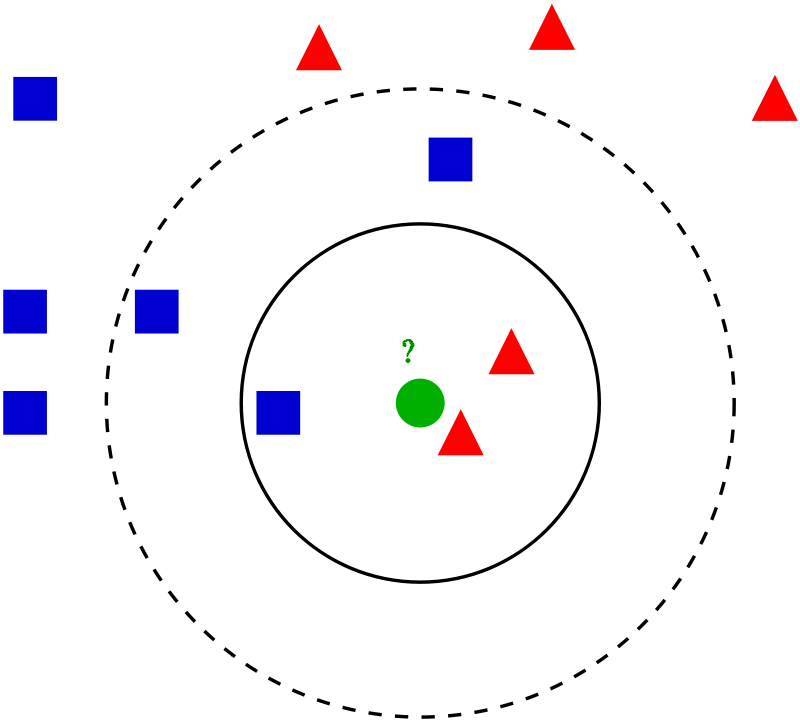
\includegraphics[width=.2\textwidth]{knn_graphic.png}
  \caption{Diagram illustrating KNN classification with example data as shapes.}
  \label{fig:knnimg}
\end{figure}

Using the data pre-processing detailed in the above section, the thirty-second audio samples were reduced to a compressed MFCC feature space. To find the highest test classification accuracy, the number of principal components was varied from 16 to 19, and the number of nearest neighbors used to classify the data was varied from 2 to 29. 

\subsection{SVM Design}
Based on the results of \cite{c7}, for our SVM we focused on fitting processed data with a linear model. A linear SVM has the goal of finding the hyperplane that produces the largest margin of separation between the categories. Two different optimization schemes, Stochastic Gradient Descent (SGD) and Adaptive Moment Estimation (ADAM), were used. Stochastic gradient descent reduces the computation load compared to normal gradient descent by randomly selecting data points each time to calculate derivatives. Adam, on the other hand, computes the adaptive learning rate for each parameter and stores the average of the exponentially decaying past gradient magnitudes. The hinge loss function shown below was used.\\
$L = \frac{1}{2} ||w||^2 + \frac{c}{n}\sum_{i=1}^{n}max(0,1-y_iw_ix_i) $\\
Twenty epochs with batch size of 30 were used. 

Linear SVM models were generated with all four databases, and the hyperparameters, including learning rate and C, were tuned for each. 

% \newline \,\,

\subsection{NN Pre-Processing and Spectrogram Generation}

While it is possible to train a Neural Network with MFCC features, we decided that with our limited amount of data, a better approach might be to use transfer learning. Transfer learning is the process of retraining the final layers of a pre-trained network to target new output classes. There are many state of the art pre-trained image classifiers available for use in the Pytorch library. To utilize these, we needed to turn our classification problem into in image classification problem. A reasonable way of doing this was converting our data stored in the .npy files into Mel spectrograms instead of extracting MFCC coefficients.

A spectrogram is a way of representing a non-periodic signal’s frequency components over time. This is done by taking a short-time Fourier transform of the data over several overlapping windows of the signal, and then stacking this data together to get the relative amplitudes of frequency components versus time. 

A Mel spectrogram adjusts the spectrogram above for human perception, which is ideal for human subjective labels like music genres. The Mel spectrum is shown in Figure \ref{fig:melspectrum}.

\begin{figure}[!hb]
\begin{center}
    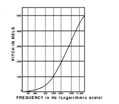
\includegraphics[width=4cm]{melspectrum.png}
\caption{Mel spectrum}
\label{fig:melspectrum}
\end{center}

\end{figure}


Thus the Mel spectrogram is simply a spectrogram except the frequencies have been converted to Mel frequencies by using the graph above. An example of a Dream pop and a Shoegaze log Mel spectrogram are shown below in Figures \ref{fig:meldreampop} and \ref{fig:melshoegaze}, respectively.


\begin{figure}[!ht]
\begin{center}
    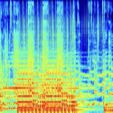
\includegraphics[width=3.5cm]{dreampop_spectrogram.png}
\caption{Log Mel spectrogram of a Dream pop song}
\label{fig:meldreampop}
\end{center}

\end{figure}


\begin{figure}[!ht]
\begin{center}
    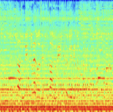
\includegraphics[width=3.5cm]{shoegaze_spectrogram.png}
\caption{Log Mel spectrogram of a Shoegaze song}
\label{fig:melshoegaze}
\end{center}
\end{figure}


Thus with converting our data to Mel spectrograms we have changed our problem to an image classification problem. These data are then easy to feed into a pre-trained network in which we adjust the final layer to target Mel spectrograms instead of standard images. 

\subsection{NN Design}

The obvious visual difference in the log Mel spectrograms shown above was good indication that an image classier would work well for a neural network. For our pre-trained network, we chose VGG16, a model that scores 92.7\% on the Imagenet database. The architecture for the VGG16 network is shown below in Figure \ref{fig:vgg16}.

\begin{figure}[!ht]
\begin{center}
    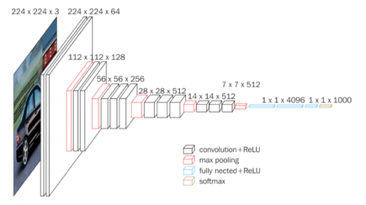
\includegraphics[width=4cm]{VGG16acc.png}
\caption{Neural Network Architecture for VGG16}
\label{fig:vgg16}
\end{center}
\end{figure}


We froze all of the layers of the VGG16 model, and replaced the final layer with our own fully connected layer to distinguish between two classes (for example Dream pop vs. Shoegaze). We then used our train and validation data to train the weights for this final layer. For this training, we used a cross entropy loss function, stochastic gradient descent with a momentum of 0.9, and a learning rate of 0.001 over 50 epochs. A system with 8 CPUs was used to reduce training time. Before any training, the base VGG16 model gave an average test accuracy for each genre comparison of 50.64\%. The full results after training are discussed below.


% \newline \,\,


\section{Results and Discussion}

The results from model training for KNN, SVM, and NN are discussed below
\newline \,\,

\par KNN Results

\begin{table}[!hb]
    \begin{center}
    \caption{KNN Classification Accuracies}{\label{tab:knn_acc}}
    \begin{tabular}{ |c|c|c| }
      Subgenres & Test Acc. & Parameters \\ 
      Shoegaze \& Dream pop & 77.49\% & 17 PC, 18 N\\
      Math vs. Post rock & 68.50\% & 19 PC, 10 N\\
      Prog. vs. Tech house & 66.50\% & 19 PC, 24 N\\
      Folk vs. Roots rock & 72.28\% & 17 PC, 5 N\\
     
    \end{tabular}\\
    \end{center}
    (PC = principal components, N = number of nearest neighbors)
\end{table}

\par When classifying songs between the sub-genres, the test accuracies ranged from 66.50\% to 77.49\%, as detailed in Table \ref{tab:knn_acc}. The complete plots of accuracies as the number of principal components and neighbors were varied is shown in Figures \ref{fig:knngraph1}-\ref{fig:knngraph4}. 
This decent accuracy range for classification indicates that a reasonable difference exists between similar sub-genres using compressed information from cepstral features. Classification was best for Dream pop vs. Shoegaze, indicating that spectral features may be a key distinguisher between those genres, while for Math rock vs. Post rock and Progressive house vs. Tech house, the classification accuracies were lower, indicating other features or methods may be needed to better distinguish those sub-genres. \newline

% <KNN Figures>

% \newline \,\,
\par SVM results 
% \vspace{\medskipamount}

\begin{table}[!ht]
    \begin{center}
    \caption{SVM Classification Accuracies}{\label{tab:svm_acc}}
    \begin{tabular}{ |c|c|c| }
     Subgenres & SVM Train & SVM Test \\ 
     Shoegaze vs. Dream pop & 72.5\% & 74.5\% \\
     Post vs. Math rock & 69.3\% & 67.1\% \\
     Progressive vs. Tech house & 65.4\% & 65.5\% \\
     Folk vs. Roots rock & 74.3\% & 65.3\% \\
    \end{tabular}\\
    \end{center}
\end{table}
\par While achieving similar maximum accuracy, the model generated with the Adam optimizer displayed a faster convergence in the loss function plot. Thus, the results reported below in Table \ref{tab:svm_acc} and Figures \ref{fig:svmtrain1}-\ref{fig:svmtrain4} are based on those models.



% <SVM Figures>

\par In general, the training and testing accuracy obtained with the data fitted with linear SVM models ranged from mid-sixty to mid-seventy percent, as detailed in Table \ref{tab:svm_acc}. The model generated from the Shoegaze and Dream pop database demonstrated the highest accuracy. The accuracy of the model on Progressive Rock and Math Rock, as well as Progressive House and Tech House, are slightly lower. However, these results are expected as they are within the range of accuracies shown in \cite{c7}. However, higher results could possibly be achieved with a non-linear model. \newline

\par NN Results 
\vspace{\medskipamount}
\par Our NN results are as follows:

\begin{table}[!hb]
\begin{center}
    \caption{NN Classification Accuracies}{\label{tab:nn_acc}}
    \begin{tabular}{ |c|c|c| }
 Subgenres & NN Train & NN Test \\ 
 Shoegaze vs. Dreamp pop &  83.40\% & 84.20\% \\
 Post vs. Math rock & 81.10\% & 80.70\% \\
 Progressive vs. Tech house & 71.30\% & 70.70\% \\
 Folk vs. Roots rock & 75.10\% & 70.50\% \\
\end{tabular}\\
\end{center}
\end{table}


\par From Table \ref{tab:nn_acc}, we can see that the accuracies are better than with the previous two models. While none of the results were greater than 90\%, the accuracies, in particular for Shoegaze vs. Dream pop and Math rock vs. Post rock were quite high, with both being better than 80\%. An accuracy vs. epoch curve for Shoegaze vs Dreampop is shown in Figure \ref{fig:nn_acc}. Comparing this with \cite{c7}, we see our results are similar, indicating the transfer learning method worked well. We notice, however, that we do not get quite as good results for the other two genre classifications, with both around 70\% accuracy. We note that there was considerably less data for these classes of sub-genres, and this is likely why we see such a stark difference in results. We speculate that with more data for each genre, and perhaps an even finer tuned model, we could achieve results upwards of 89\% similar to \cite{c7}.

% <NN Figure>



% \newline \,\,



\section{Conclusion and Future Work}

In the discussion of our results above, we can see that the methods of KNN, SVM, and NN applied to the classification problem of closely related music sub-genres does work quite well. However, a key constraint to these results is the quantity of labeled data. Where less data was publicly available, the results suffered. Therefore, we reasonably conclude that while our results are good, they will likely get better with the addition of more data.   

Furthermore, we note that neural networks are clearly the superior model for classifying closely related music sub-genres. This result is likely because the model was built on top of a pre-trained and highly accurate image classifier. Nonetheless, this method of transfer learning produced better results across the board even with limited amounts of data. 

There are a number of improvements that could be made for future work in this domain. First and most importantly would be to use a different audio collection strategy. While the Spotify API is convenient, the restriction to random 30 second samples is an extreme hindrance to the flexibility of data collection. If we had more control of this process, our accuracies would likely increase because, at the moment, nothing is stopping 30 seconds of mostly silence from appearing in a sample. Second, as mentioned previously, a linear SVM may not produce the best classification, so exploring non-linear SVM might yield higher accuracies. Third, considering that transfer learning worked the best, it is a good idea to explore different pre-trained models. Furthermore, using the collected Spotify-defined audio features in our database to supplement our audio features could also provide an additional boost in accuracy. Lastly, extending our classification to a multi-class system would be informative. Instead of doing binary comparisons, we could pick $N$ closely related sub-genres and classify the difference between all of them. 

To conclude, machine learning methods, in particular neural networks, work well at classifying closely related music sub-genres. However, more work needs to be done to push these results to greater than 90\% accuracy. 

\section*{ACKNOWLEDGMENT}

The authors would like to thank Mert Pilanci and Yifei Wang for their guidance on this project.



\begin{thebibliography}{99}



\bibitem{c1} Cataltepe, Z., Yaslan, Y. & Sonmez, A. Music Genre Classification Using MIDI and Audio Features. EURASIP J. Adv. Signal Process. 2007, 036409 (2007). https://doi.org/10.1155/2007/36409

\bibitem{c2} Bahuleyan, Hareesh. "Music genre classification using machine learning techniques." arXiv preprint arXiv:1804.01149 (2018)..

\bibitem{c3} Haggblade, Michael, Yang Hong, and Kenny Kao. "Music genre classification." Department of Computer Science, Stanford University (2011). 

\bibitem{c4} Choi, Keunwoo, et al. "Convolutional recurrent neural networks for music classification." 2017 IEEE International Conference on Acoustics, Speech and Signal Processing (ICASSP). IEEE, 2017.


\bibitem{c5} Montgomerie, Adam.  Music genre classification of mel-spectrograms using convolutional and
recurrent neural networks. 2020

\bibitem{c6}  Antonio Caparrini, Javier Arroyo, Laura Pérez-Molina & Jaime Sánchez-Hernández (2020) Automatic subgenre classification in an electronic dance music taxonomy, Journal of New Music Research, 49:3, 269-284, DOI: 10.1080/09298215.2020.1761399



\bibitem{c7} R. J. M. Quinto, R. O. Atienza and N. M. C. Tiglao, "Jazz music sub-genre classification using deep learning," TENCON 2017 - 2017 IEEE Region 10 Conference, 2017, pp. 3111-3116, doi: 10.1109/TENCON.2017.8228396.


\bibitem{c8} https://indiepanda.net/what-do-record-labels-look-for/


\end{thebibliography}

\newpage
\section{Appendix}

% KNN Figures
\par KNN Parameter Tuning Plots
\begin{figure}[H]
    \centering
    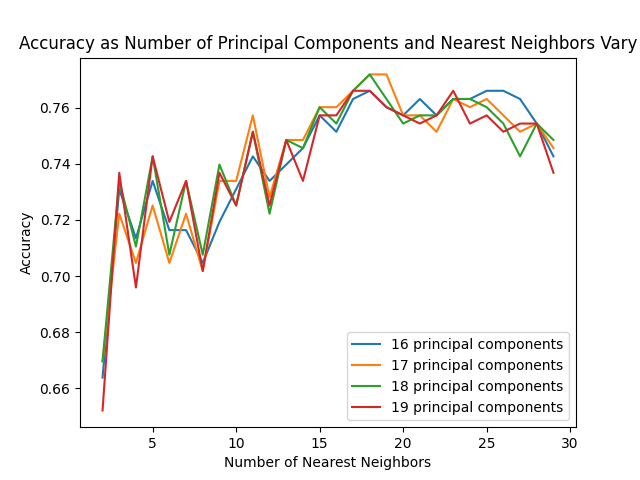
\includegraphics[width=.8\linewidth]{knnplot_dpsg.png}
    \caption{Plot showing changes in KNN classifier accuracy as the number of principal components and number of neighbors used for classification were varied for Shoegaze vs. Dream pop}
    \label{fig:knngraph1}
\end{figure}
\begin{figure}[H]
    \centering
    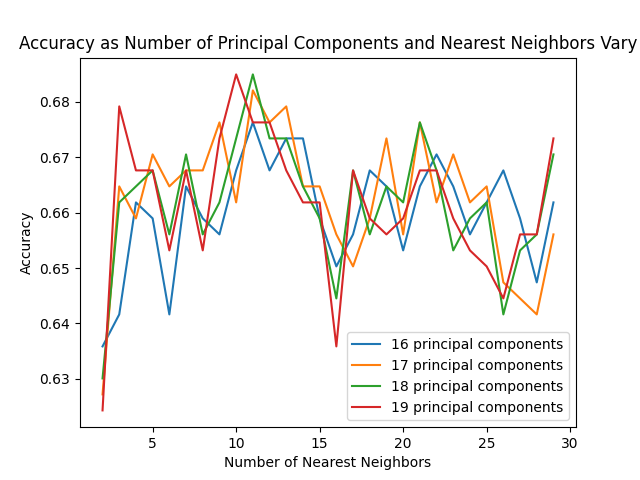
\includegraphics[width=.8\linewidth]{knnplot_mrpr.png}
    \caption{Plot showing changes in KNN classifier accuracy as the number of principal components and number of neighbors used for classification were varied for Math vs. Post Rock}
    \label{fig:knngraph2}
\end{figure}
\begin{figure}[H]
    \centering
    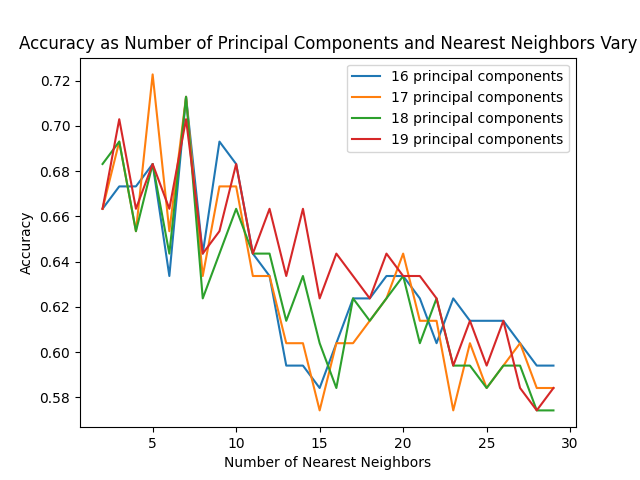
\includegraphics[width=.8\linewidth]{knnplot_frrr.png}
    \caption{Plot showing changes in KNN classifier accuracy as the number of principal components and number of neighbors used for classification were varied for Folk vs. Roots Rock}
    \label{fig:knngraph3}
\end{figure}
\begin{figure}[H]
    \centering
    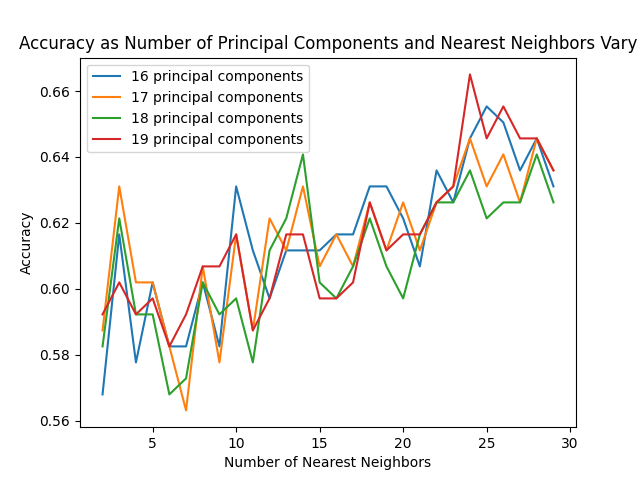
\includegraphics[width=.8\linewidth]{knnplot_thph.png}
    \caption{Plot showing changes in KNN classifier accuracy as the number of principal components and number of neighbors used for classification were varied for Tech vs. Prog. House}
    \label{fig:knngraph4}
\end{figure}

% \newpage
% SVM Figures
\par SVM Training Loss Plots
\begin{figure}[H]
\centering
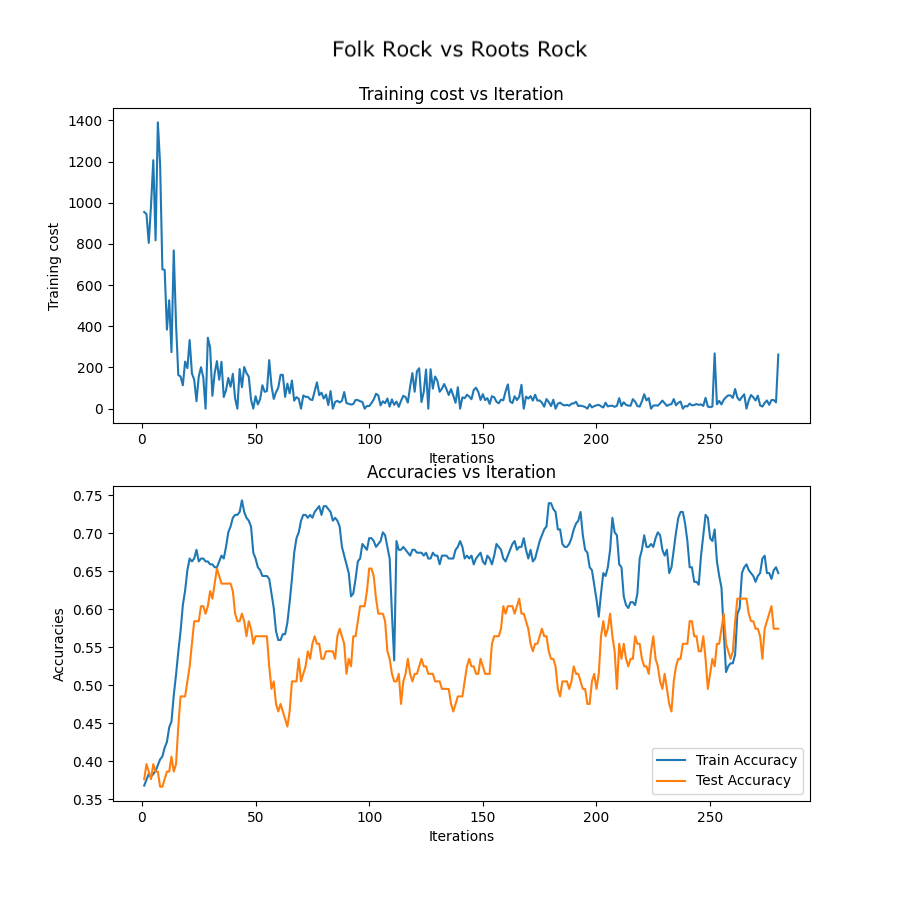
\includegraphics[width=.75\linewidth]{frrr_svm.png}
\caption{Folk Rock vs. Roots Rock}
\label{fig:svmtrain1}
\end{figure}
\begin{figure}[H]
\centering
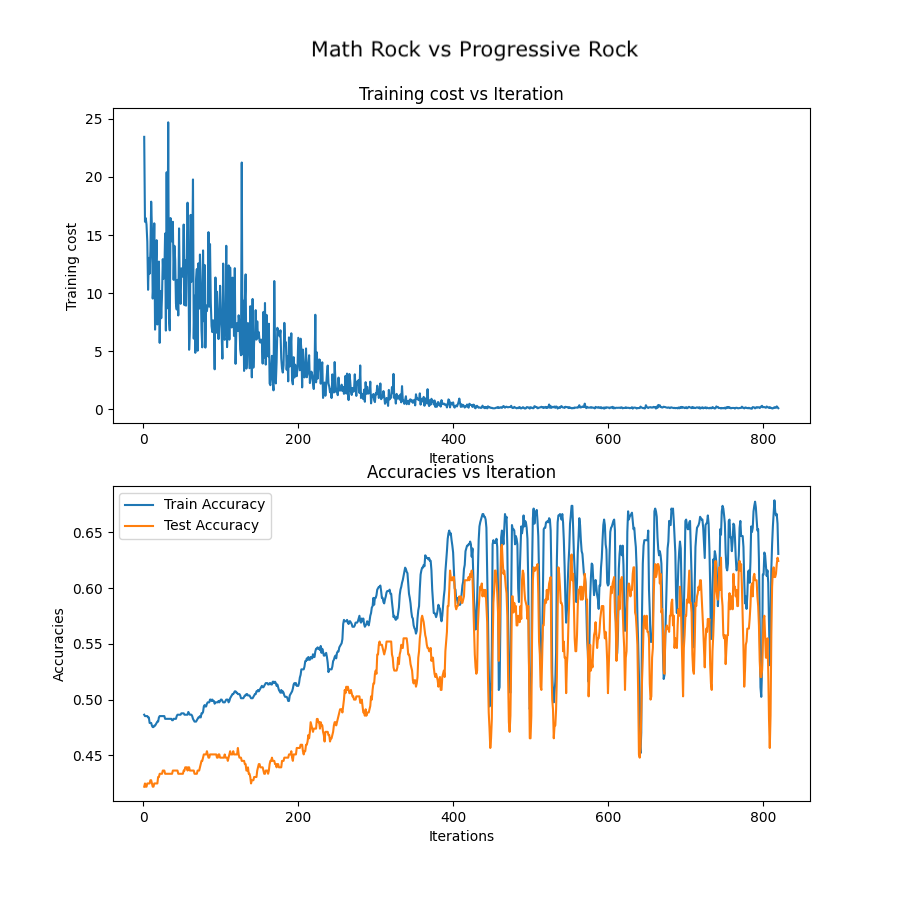
\includegraphics[width=.75\linewidth]{mrpr_svm.png}
\caption{Math Rock vs. Progressive Rock}
\label{fig:svmtrain2}
\end{figure}
\begin{figure}[H]
\centering
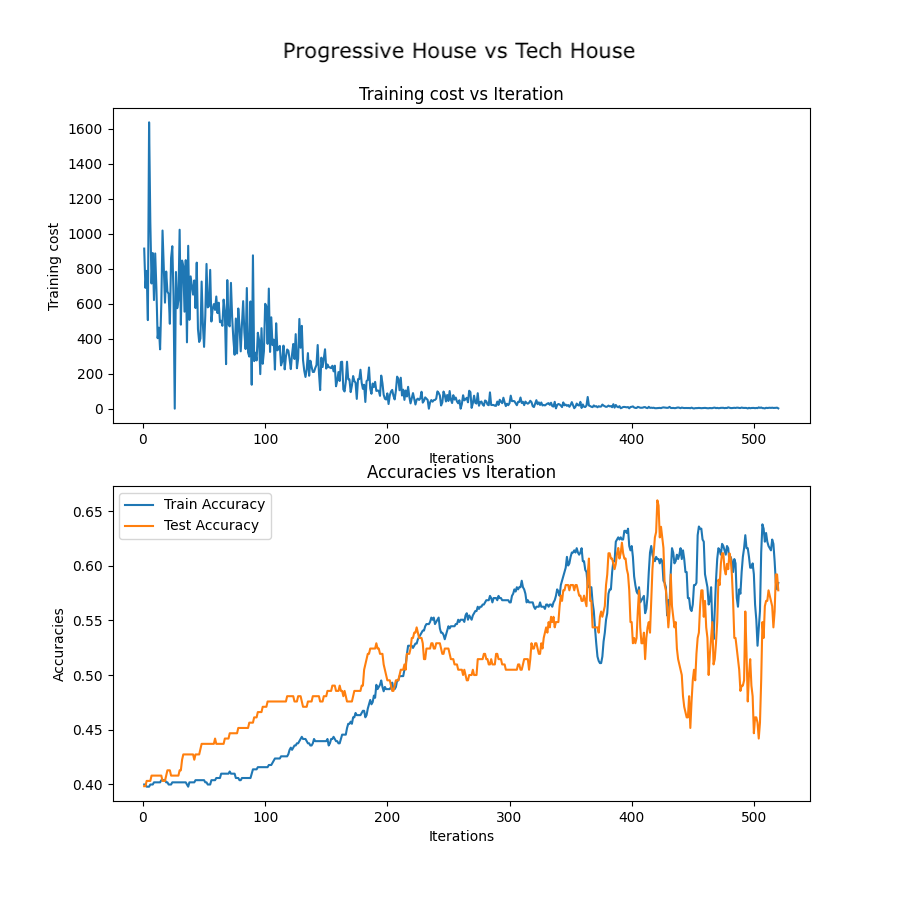
\includegraphics[width=.75\linewidth]{phth_svm.png}
\caption{Progressive House vs. Tech House}
\label{fig:svmtrain3}
\end{figure}
\begin{figure}[H]
\centering
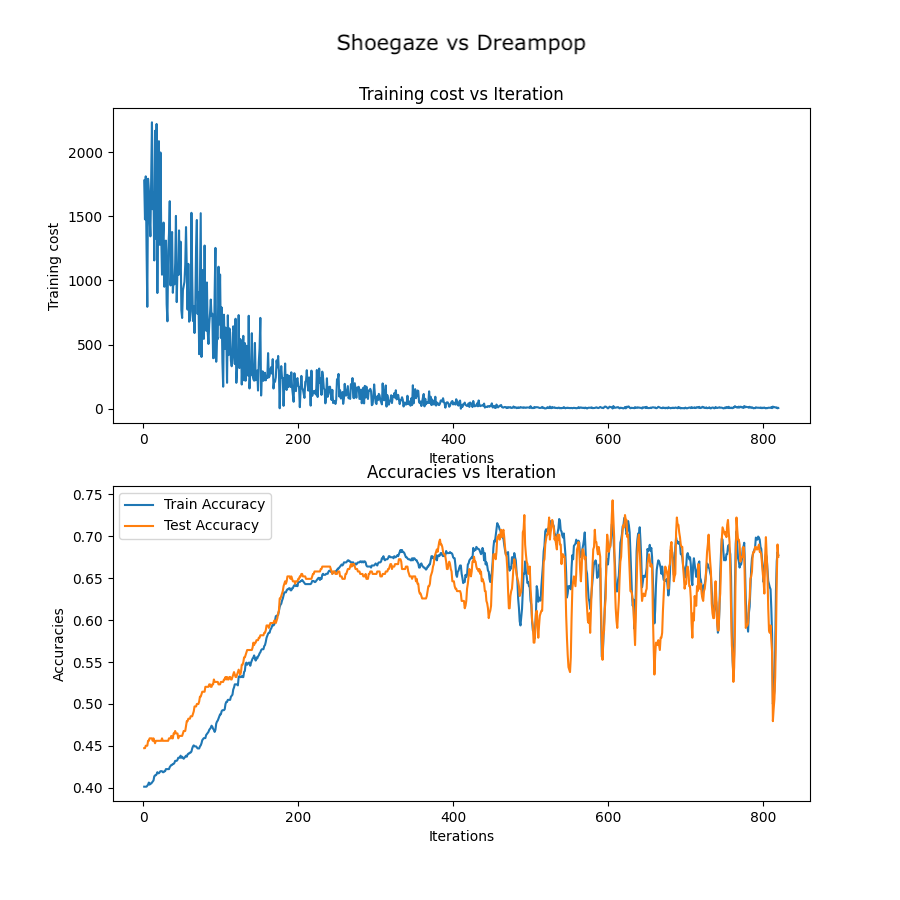
\includegraphics[width=.75\linewidth]{sgdp_svm.png}
\caption{Shoegaze vs. Dream pop}
\label{fig:svmtrain4}
\end{figure}

% NN Figures
\par NN Training Accuracy Plot
\begin{figure}[H]
\centering
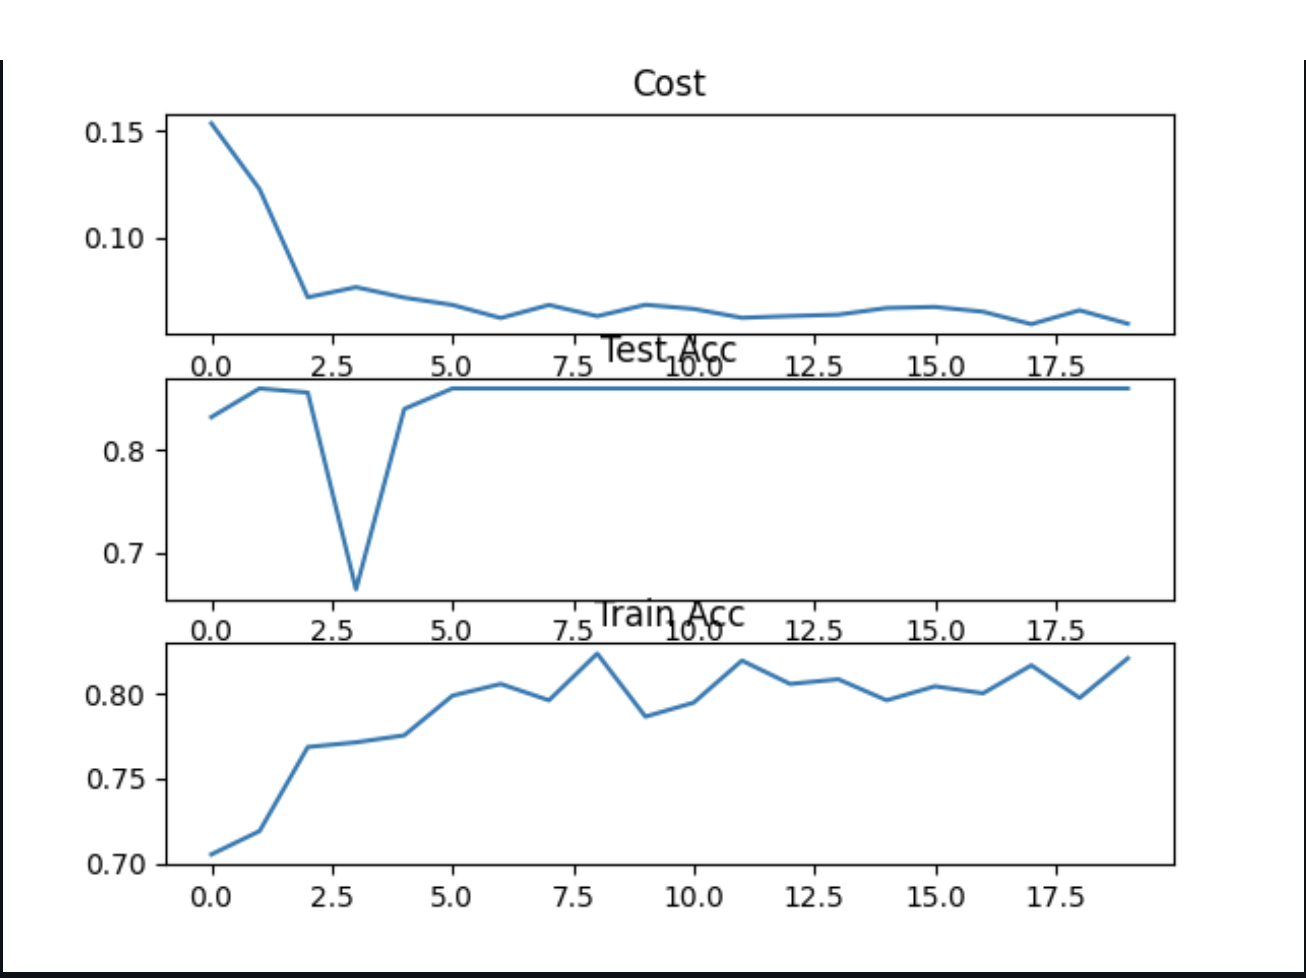
\includegraphics[width=7cm]{nn_train.png}
\caption{Accuracy vs. Epoch for Dreampop vs. Shoegaze}
\label{fig:nn_acc}
\end{figure}

\end{document}
